%%%%%%%%%%%%%%%%%%%%%%%%%%%%%%%%%%%%%%%%%
%%%%%                               %%%%%
%%%%%     STATISTICS OF CHAOTIC     %%%%%
%%%%%                               %%%%% 
%%%%%%%%%%%%%%%%%%%%%%%%%%%%%%%%%%%%%%%%% 

\begin{frame}[t, c]{}{}
  \begin{minipage}{.48\textwidth}
    \centering
    \begin{tikzpicture}
      \node[state] (s1) {\( \bm{s}_1 \)};
      \node[state, below right of=s1] (s2) {\( \bm{s}_2 \)};
      \node[state, below left of=s1] (s4) {\( \bm{s}_4 \)};
      \node[state, below left of=s2] (s3) {\( \bm{s}_3 \)};
      
      \draw (s1) edge[loop above] node {\(l_{11}\)} (s1);
      \draw (s1) edge[bend left] node {\(l_{21}\)}  (s2);
      
      \draw (s2) edge[loop right]  node {\(l_{22}\)} (s2);
      \draw (s2) edge[bend left]  node {\(l_{32}\)} (s3);
      
      \draw (s3) edge[bend left]  node {\(l_{43}\)} (s4);
      \draw (s3) edge[loop below]  node {\(l_{33}\)} (s3);
      
      \draw (s4) edge[bend left]  node {\(l_{14}\)} (s1);
      \draw (s4) edge[loop left]  node {\(l_{44}\)} (s4);
      
    \end{tikzpicture}
  \end{minipage}%
  \hfill
  \begin{minipage}{.48\textwidth}
    \centering
    {
      \Large\textbf{Part II}
    }
    
    \bigskip
    
    \rule{\textwidth}{0.001\textwidth}
    
    \bigskip
    
    {
      \large
      \textbf{Statistics of chaotic}
    }
    
    \medskip
    
    \begin{itemize}
    \item Problem formulation:
      \begin{itemize}
      \item[\(	\hookrightarrow \)] State space partition
      \item[\(	\hookrightarrow	\)] Cluster-based Reduced Order Modeling
      \end{itemize}
      
      \medskip
      
    \item Practical usage:
      \begin{itemize}
      \item[\(	\hookrightarrow	\)] Probabilistic model
      \item[\(	\hookrightarrow \)] Statistics of chaos
      \end{itemize}
      
    \end{itemize}
    
  \end{minipage}
\end{frame}

\begin{frame}[t, c]{Statistics of chaotic}{Overview}
  \begin{minipage}{.28\textwidth}
    \centering
    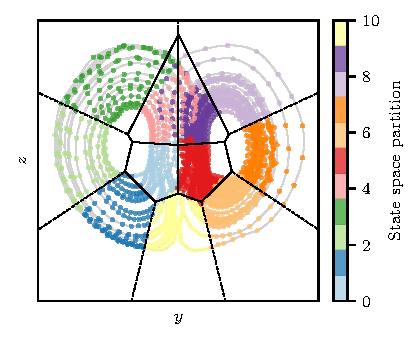
\includegraphics[width=\textwidth]{voronoi_diagram}
  \end{minipage}%
  \hfill
  \begin{minipage}{.68\textwidth}
    \begin{block}{}
      \centering
      \textbf{Cluster-based Reduced-Order Modeling}
    \end{block}
    
    \medskip
    
    \begin{itemize}
    \item \textbf{Aim:} Coarse-gain probabilistic model of the dynamics
      \begin{itemize}
      \item[\(	\hookrightarrow	\)] Linear model for the probability density function.
      \item[\(	\hookrightarrow	\)] Statistical properties of the system.
      \end{itemize}
      
      \medskip
      
    \item \textbf{How:} From continuous to symbolic dynamics.
      \begin{itemize}
      \item[\(	\hookrightarrow	\)] State-space partitionning using \underline{k-means}.
      \item[\(	\hookrightarrow	\)] Maximum likelihood estimation of the transition probability from cluster \( \bm{c}_i \) to cluster \( \bm{c}_j \).
      \end{itemize}
    \end{itemize}
  \end{minipage}
  
  \vspace{1cm}
\end{frame}

\begin{frame}[t, c]{Statistics of chaotic}{State-space partitionning}
  \begin{minipage}{.68\textwidth}
    \begin{itemize}
    \item Given a set of \( n \) observations \( (\bm{x}_1, \bm{x}_2, \cdots, \bm{x}_n) \), partition the data into \( k \) sets \( \bm{C} = \left\{ \bm{C}_1, \bm{C}_2, \cdots, \bm{C}_k \right\} \).
      
      \medskip
      
    \item To do so, \underline{k-means} aims to minimize the \emph{within-cluster sum of squares}
      % 
      \[
        \minimize_{\bm{C}} \sum_{i=1}^k \sum_{\bm{x} \in \bm{C}_i} \| \bm{x} - \bm{c}_i \|^2
      \]
      % 
      where \( \bm{c}_i \) is the centroid of the i\textsuperscript{th} cluster \( \bm{C}_i \).
    \end{itemize}
  \end{minipage}%
  \hfill
  \begin{minipage}{.28\textwidth}
    \centering
    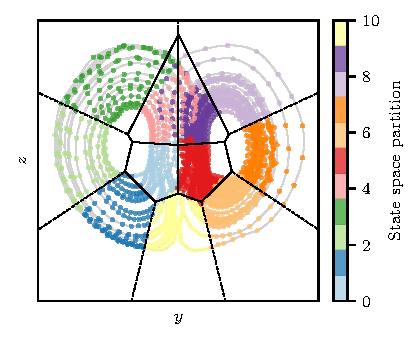
\includegraphics[width=\textwidth]{voronoi_diagram}
  \end{minipage}
  
  \vspace{1cm}
\end{frame}

\begin{frame}[t, c]{Statistics of chaotic}{State-space partitionning}
  \centering
  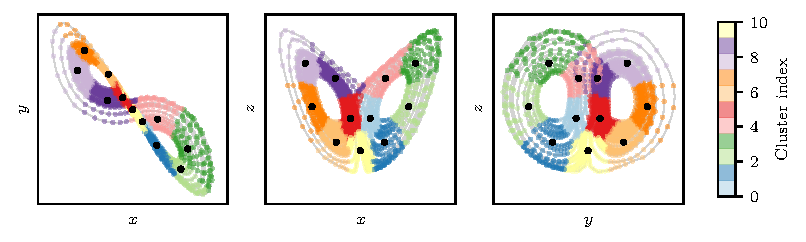
\includegraphics[width=\textwidth]{clustered_attractor}
  
  \vspace{1cm}
\end{frame}

\begin{frame}[t, c]{Statistics of chaotic}{Symbolic dynamics}
  \begin{minipage}{.48\textwidth}
    \centering
    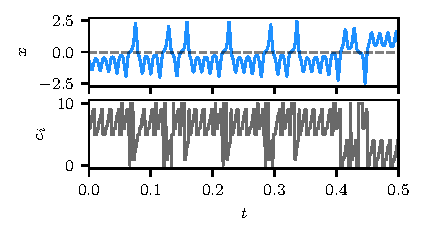
\includegraphics[width=\textwidth]{dns_crom_time_series}
  \end{minipage}%
  \hfill
  \begin{minipage}{.48\textwidth}
    \begin{itemize}
    \item Symbolic dynamics are obtained by looking at the evolution of the cluster index \( c(t) \).
      % \begin{itemize}
      % \item[\(	\hookrightarrow	\)] Dynamics on a finite set of \( k \) symbols.
      % \end{itemize}
      
      \medskip
      
    \item These dynamics can easily be modeled using a Markov chain.
      % \begin{itemize}
      % \item[\(	\hookrightarrow	\)] Transition matrix obtained from maximum likelihood estimation.
      % \end{itemize}
      
    \end{itemize}
  \end{minipage}
  
  \vspace{1cm}
\end{frame}

\begin{frame}[t, c]{Statistics of chaotic}{Markov chain model}
  \begin{minipage}{.68\textwidth}
    \begin{itemize}
    \item Using MLE, a Markov chain model
      % 
      \[
        \bm{p}_{k+1} = \bm{Lp}_k
      \]
      % 
      is identified where the i\textsuperscript{th} entry of \( \bm{p}_k \) describes the probability of being in cluster \( \bm{C}_i \) at time \( t = k \Delta T \).
      
      \medskip
      
    \item \( l_{ij} \) encodes the transition probability from cluster \( \bm{C}_j \) to cluster \( \bm{C}_i \) after one step.

    \end{itemize}
  \end{minipage}%
  \hfill
  \begin{minipage}{.28\textwidth}
    \centering
    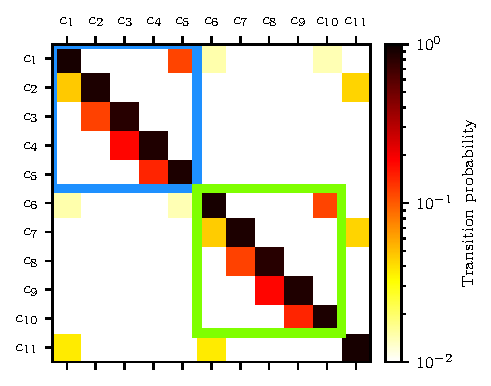
\includegraphics[width=\textwidth]{CROM_transition_matrix} \\
    
    {\small
      Transition matrix \( \bm{L} \).
    }
  \end{minipage}
  
  \vspace{1cm}
\end{frame}

\begin{frame}[t, c]{Statistics of chaotic}{Markov chain model}
  \begin{minipage}{.68\textwidth}
    \begin{itemize}
      
    \item Existence of two ``mega-clusters'' corresponding to the clockwise and counter-clockwise rotation.
      
      \medskip
      
    \item When reaching the last cluster, the system to randomly switch from one side of the attractor to the other.
    \end{itemize}
  \end{minipage}%
  \hfill
  \begin{minipage}{.28\textwidth}
    \centering
    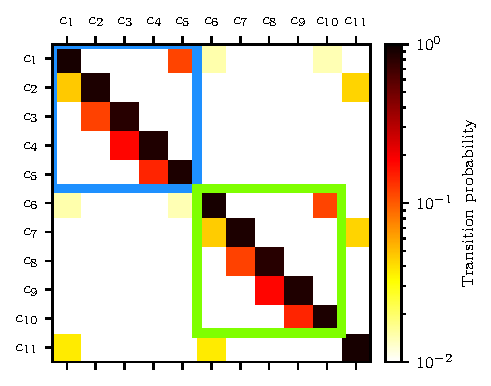
\includegraphics[width=\textwidth]{CROM_transition_matrix} \\
    
    {\small
      Transition matrix \( \bm{L} \).
    }
  \end{minipage}
  
  \vspace{1cm}
\end{frame}

\begin{frame}[t, c]{Statistics of chaotic}{Markov chain model}
  \centering
  \begin{tikzpicture}
    \node[state] (s2) at (36+0:2) {\( \bm{c}_2 \)};
    \node[state] (s3) at (36+72:2) {\( \bm{c}_3 \)};
    \node[state] (s4) at (36+144:2){\( \bm{c}_4 \)};
    \node[state] (s5) at (36+216:2) {\( \bm{c}_5 \)};
    \node[state] (s1) at (36+288:2) {\( \bm{c}_1 \)};
    
    \node[state, xshift=8cm] (s7) at (180-36:2) {\( \bm{c}_7 \)};
    \node[state, xshift=8cm] (s8) at (180-72-36:2) {\( \bm{c}_8 \)};
    \node[state, xshift=8cm] (s9) at (180-144-36:2) {\( \bm{c}_9 \)};
    \node[state, xshift=8cm] (s10) at (180-216-36:2) {\( \bm{c}_{10} \)};
    \node[state, xshift=8cm] (s6) at (180-288-36:2) {\( \bm{c}_6 \)};
    
    \node[state, xshift=4cm] (s11) at (0, 0) {\( \bm{c}_{11} \)};
    
    \draw (s1) edge[bend right, red] node {}  (s2);
    \draw (s1) edge[bend right, red!50] node {} (s11);
    \draw (s1) edge[bend right, red!25] node {} (s6);
    
    \draw (s2) edge[bend right, red] node {} (s3);
    
    \draw (s3) edge[bend right, red] node {} (s4);
    
    \draw (s4) edge[bend right, red] node {} (s5);
    
    \draw (s5) edge[bend right, red] node {} (s1);
    
    
    \draw (s6) edge[bend left, red] node {} (s7);
    \draw (s6) edge[bend left, red!50] node {} (s11);
    \draw (s6) edge[bend left, red!25] node {} (s1);
    
    \draw (s7) edge[bend left, red] node {} (s8);
    
    \draw (s8) edge[bend left, red] node {} (s9);
    
    \draw (s9) edge[bend left, red] node {} (s10);
    
    \draw (s10) edge[bend left, red] node {} (s6);
    
    \draw (s11) edge[bend right, red] node {} (s2);
    \draw (s11) edge[bend left, red] node {} (s7);
    
    \node at (0, 0) {\textsc{Clockwise}};
    \node at (8, 0) {\textsc{Anticlockwise}};
    
  \end{tikzpicture}
  
  \vspace{1cm}
\end{frame}

\begin{frame}[t, c]{Statistics of chaotic}{Statistical analysis}
  \begin{minipage}{.68\textwidth}
    \begin{itemize}
    \item Eigenspectrum of \( \bm{L} \) encodes the diffusion of the probability density function.
      
      \bigskip
      
    \item Eigenvector \( \bm{p}^{\infty} \) associated to \( \lambda_1 = 1 \) characterizes the invariant measure (i.e. the long-time/ensemble average distribution of \( \bm{p} \)).
    \end{itemize}
    
    \bigskip
    
    \centering
    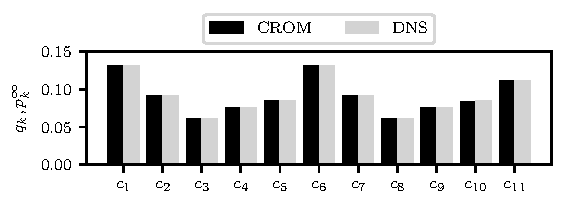
\includegraphics[width=.8\textwidth]{probability_distribution}
  \end{minipage}%
  \hfill
  \begin{minipage}{.28\textwidth}
    \centering
    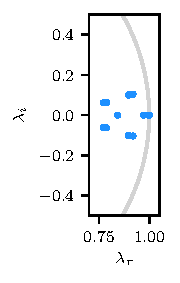
\includegraphics[height=.666\textheight]{CROM_eigenspectrum}
  \end{minipage}
  
  \vspace{1cm}
\end{frame}

\begin{frame}[t, c]{Statistics of chaotic}{Statistical analysis}
  \begin{minipage}{.68\textwidth}
    \begin{itemize}
    \item How fast the p.d.f.\ diffuses is related to the ratio \( \nicefrac{\vert \lambda_2 \vert}{\vert \lambda_1 \vert} \).
      \begin{itemize}
      \item[\( \hookrightarrow	\)] The larger it is, the faster the p.d.f.\ converges to its invariant measure.
      \end{itemize}
      
      \medskip
      
    \item \( \vert \lambda_2 \vert^k \) provides an estimate of how far in time we can predict.
      \begin{itemize}
      \item[\( \hookrightarrow	\)] Our prediction horizon is only one characteristic time-scale.
      \end{itemize}
    \end{itemize}
    
    \medskip
    
    \centering
    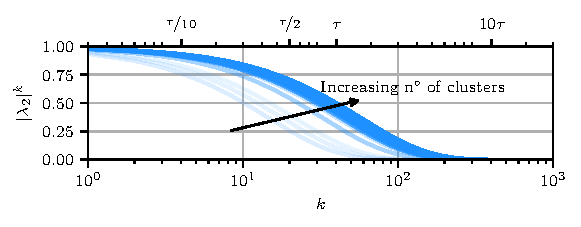
\includegraphics[width=.8\textwidth]{convergence_crom}
  \end{minipage}%
  \hfill
  \begin{minipage}{.28\textwidth}
    \centering
    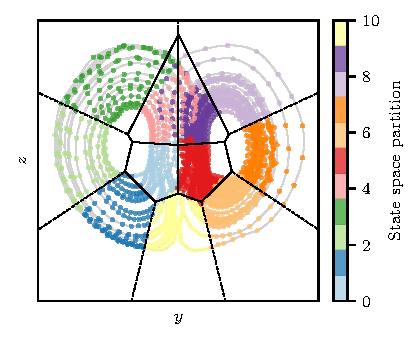
\includegraphics[width=\textwidth]{voronoi_diagram}
  \end{minipage}
  
  \vspace{1cm}
\end{frame}
